All results are on the test sessions. ``Initial'' is the initial Seq2Seq-GRU retrained on the corrected data with the same protocol as the final model.

\subsection{Headline: RTT with session-level uncertainty}
The test windows of one session overlap and share its regime, so the unit of independent evidence is the session. Table~\ref{tab:boot} and Fig.~\ref{fig:bootstrap} compare the two ensembles with a paired bootstrap over whole test sessions (2000 replicates, script \texttt{fr\_bootstrap.py}). The interval score improves significantly on all six links, and DS2S-E has the lower interval score in each of the \BSnSessTot{} test sessions. The MAE improves significantly on five links and is inconclusive on OneWeb UL. The RMSE improves significantly on Starlink DL and both 5G links and is inconclusive on the other three. No change is significantly worse. Coverage is close to 0.95 everywhere except Starlink UL, where both models under-cover slightly.

\begin{table}[htbp]
\centering
\caption{RTT on the test sessions, averaged over 0.2--3\,s, for the three-seed ensembles S2S-E (initial) and DS2S-E (final). Changes with 95\% session-bootstrap intervals. Bold: the interval excludes zero. MAE uses the median of DS2S-E, RMSE the means. IS and PICP refer to the calibrated 95\% interval.}
\label{tab:boot}
\resizebox{\linewidth}{!}{%
\begin{tabular}{l rrr rrr rrr cc}
\toprule
 & \multicolumn{3}{c}{Interval score (ms)} & \multicolumn{3}{c}{MAE (ms)} & \multicolumn{3}{c}{RMSE (ms)} & \multicolumn{2}{c}{PICP} \\
\cmidrule(lr){2-4}\cmidrule(lr){5-7}\cmidrule(lr){8-10}\cmidrule(lr){11-12}
Link & S2S-E & DS2S-E & $\Delta$\% [95\% CI] & S2S-E & DS2S-E & $\Delta$\% [95\% CI] & S2S-E & DS2S-E & $\Delta$\% [95\% CI] & S2S-E & DS2S-E \\
\midrule
\tabinput{data/tab_main_boot.tex}
\bottomrule
\end{tabular}}
\end{table}

\begin{figure}[htbp]
  \centering
  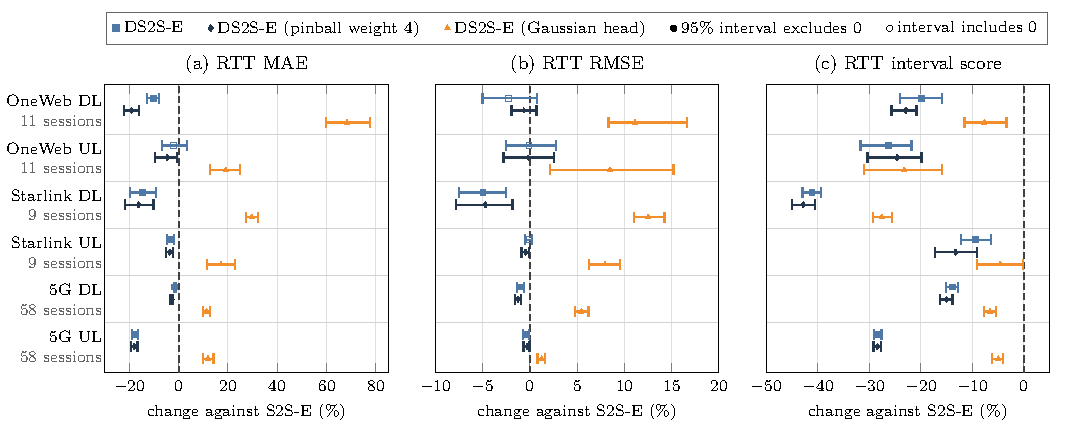
\includegraphics[width=\linewidth]{figs_pdf/fr_bootstrap.pdf}
  \caption{Session-level bootstrap of the RTT change of DS2S-E against S2S-E (2000 replicates). Marker: bootstrap median. Bar: 95\% percentile interval. Filled: the interval excludes zero. Negative values favor DS2S-E.}
  \label{fig:bootstrap}
\end{figure}

A bootstrap over windows would give intervals \BSWidRatioLo{} to \BSWidRatioHi{} times narrower and would call two inconclusive changes significant. Leaving out any one test session moves the interval-score change by at most \BSLooMax{} points. A Wilcoxon test over sessions confirms the MAE gain at the 1\% level on five links (the final model wins \SessWinsTotal{} of \SessNTotal{} sessions). Table~\ref{tab:main} adds the seed spread of the single models, and Fig.~\ref{fig:hzoom} shows the errors per horizon.

\begin{table}[htbp]
\centering
\caption{RTT results on the test sessions, averaged over the 15 steps (0.2--3\,s). Mean $\pm$ standard deviation over 3 seeds, and 3-seed ensembles. MAE, RMSE, and MIS in ms. MIS is the calibrated 95\% interval score (split conformal for Initial, CQR for Final).}
\label{tab:main}
\scriptsize
\setlength{\tabcolsep}{3pt}
\begin{tabular}{llccccc}
\toprule
Link & Model & MAE & RMSE & $R^2$ & MIS & PICP \\
\midrule
\tabinput{data/tab_main.tex}
\bottomrule
\end{tabular}
\end{table}

\begin{figure}[htbp]
  \centering
  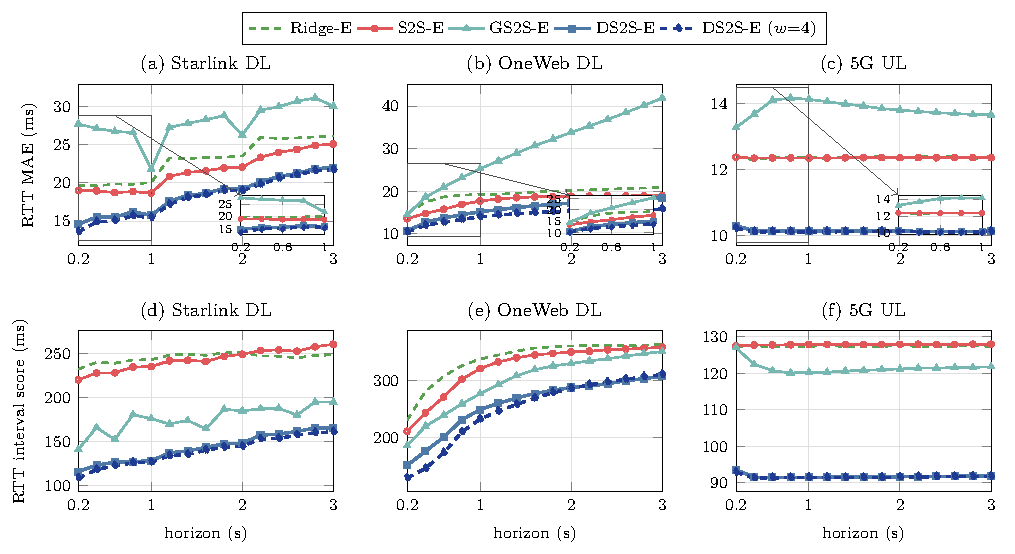
\includegraphics[width=\linewidth]{figs_pdf/fr_hzoom.pdf}
  \caption{RTT MAE (top) and calibrated 95\% interval score (bottom) per horizon on three links. DS2S-E ($w{=}4$) is the final model with pinball weight 4 (Section~\ref{sec:robust}). Insets: 0.2 to 1\,s.}
  \label{fig:hzoom}
\end{figure}

\subsection{Comparison with the Modeling Dynamics report}
Table~\ref{tab:isproto} shows why the previous evaluation could not see this gain. With intervals from the quantiles of the test residuals, the method of the previous report, the two models are within about 2\% of each other on every link, because both intervals then have a constant width. With intervals calibrated on held-out sessions, the final model changes the interval score by \ChgMISWorst\% to \ChgMISBest\% (seed means). Table~\ref{tab:y2} gives the previous ``aggregate'' (mean over the three targets and 15 steps) next to the printed numbers. The retrained initial model matches the MAE and RMSE of the Modeling Dynamics report closely. The $R^2$ differs on OneWeb UL because of A4 and on Starlink DL because the causal inputs remove the leaked signal (A3).

\begin{table}[htbp]
\centering
\caption{RTT interval score (ms, seed means) with the earlier method (test-residual quantiles around the mean) and with intervals calibrated on validation sessions.}
\label{tab:isproto}
\small
\begin{tabular}{lrrrrrr}
\toprule
 & \multicolumn{3}{c}{Earlier method} & \multicolumn{3}{c}{Calibrated} \\
\cmidrule(lr){2-4}\cmidrule(lr){5-7}
Link & Initial & Final & $\Delta$\% & Initial & Final & $\Delta$\% \\
\midrule
\tabinput{data/tab_isproto.tex}
\bottomrule
\end{tabular}
\end{table}

\begin{table}[htbp]
\centering
\caption{Aggregate in the style of the Modeling Dynamics report (mean over RTT, jitter, and loss and over the 15 steps). MIS (Initial method) uses quantiles of the test residuals. MIS (calibrated) uses intervals calibrated on validation sessions.}
\label{tab:y2}
\scriptsize
\begin{tabular}{llccccc}
\toprule
Link & Source & MAE & RMSE & $R^2$ & MIS (Initial method) & MIS (calibrated) \\
\midrule
\tabinput{data/tab_y2compare.tex}
\bottomrule
\end{tabular}
\end{table}

\subsection{Which step helps?}
Table~\ref{tab:ablation} adds the final steps one at a time. The residual decoder (Step 1) and the causal pipeline with context features (Step 2) do not improve the MAE. On OneWeb DL they make it worse, because a squared-error model anchored on a spiky last value follows the spikes. Step 2 lowers the RMSE slightly on most links (up to 4.5\% on Starlink DL). The gains in MAE and interval score come from Step 3, the distributional heads. The ensemble (Step 4) adds up to 6.4 further points (Starlink DL MAE).

\begin{table}[htbp]
\centering
\caption{Ablation: change (\%) of RTT MAE, RMSE, and calibrated interval score (MIS) relative to the retrained initial model (seed means, the last row compares the final ensemble with the initial seed mean). Negative is better.}
\label{tab:ablation}
\scriptsize
\setlength{\tabcolsep}{2pt}
\resizebox{\linewidth}{!}{%
\begin{tabular}{l*{18}{r}}
\toprule
 & \multicolumn{3}{c}{OneWeb DL} & \multicolumn{3}{c}{OneWeb UL} & \multicolumn{3}{c}{Starlink DL} & \multicolumn{3}{c}{Starlink UL} & \multicolumn{3}{c}{5G DL} & \multicolumn{3}{c}{5G UL} \\
\cmidrule(lr){2-4}\cmidrule(lr){5-7}\cmidrule(lr){8-10}\cmidrule(lr){11-13}\cmidrule(lr){14-16}\cmidrule(lr){17-19}
Steps & MAE & RMSE & MIS & MAE & RMSE & MIS & MAE & RMSE & MIS & MAE & RMSE & MIS & MAE & RMSE & MIS & MAE & RMSE & MIS \\
\midrule
\tabinput{data/tab_ablation.tex}
\bottomrule
\end{tabular}}
\end{table}

\subsection{Simple references}
Table~\ref{tab:baselines} adds the references that the initial study did not have. Persistence is a poor RTT forecast at 5\,Hz because single pings are noisy. A tuned linear model on the final features (Ridge-E) is within one point of the initial network on RMSE skill on four links. On Starlink DL a repeat of the value one second earlier already has 28\% skill, which reflects the one-second sawtooth. The final ensemble has the lowest MAE and the highest skill on every link (tied on 5G UL). Ridge on the initial features fails on 5G UL because of unclipped logger sentinels.

\begin{table}[htbp]
\centering
\caption{RTT MAE (ms) and RMSE skill against persistence (\%, higher is better) for the references and the neural models (seed means).}
\label{tab:baselines}
\scriptsize
\setlength{\tabcolsep}{3pt}
\begin{tabular}{l*{12}{r}}
\toprule
 & \multicolumn{2}{c}{OneWeb DL} & \multicolumn{2}{c}{OneWeb UL} & \multicolumn{2}{c}{Starlink DL} & \multicolumn{2}{c}{Starlink UL} & \multicolumn{2}{c}{5G DL} & \multicolumn{2}{c}{5G UL} \\
\cmidrule(lr){2-3}\cmidrule(lr){4-5}\cmidrule(lr){6-7}\cmidrule(lr){8-9}\cmidrule(lr){10-11}\cmidrule(lr){12-13}
Method & MAE & skill & MAE & skill & MAE & skill & MAE & skill & MAE & skill & MAE & skill \\
\midrule
\tabinput{data/tab_baselines.tex}
\bottomrule
\end{tabular}
\end{table}

\subsection{Jitter and loss}
Table~\ref{tab:targets} gives the jitter and loss results. Point accuracy is similar for both models, with exceptions in both directions. The calibrated interval scores of the final model are lower on every link and target, often by a large factor (Starlink DL jitter: 2.8 against 8.5). Jitter and loss are one-second iperf reports with long runs of zeros and rare large values, the case where input-dependent intervals help most.

\begin{table}[htbp]
\centering
\caption{Jitter (ms) and loss (\%) on the test sessions (seed means, OneWeb UL omitted because both are zero in every row).}
\label{tab:targets}
\scriptsize
\begin{tabular}{llcccccc}
\toprule
 & & \multicolumn{3}{c}{Jitter} & \multicolumn{3}{c}{Loss} \\
\cmidrule(lr){3-5}\cmidrule(lr){6-8}
Link & Model & MAE & RMSE & MIS & MAE & RMSE & MIS \\
\midrule
\tabinput{data/tab_targets.tex}
\bottomrule
\end{tabular}
\end{table}
